\documentclass[11pt, oneside]{article}   	% use "amsart" instead of "article" for AMSLaTeX format
\usepackage[margin=1in]{geometry}                		% See geometry.pdf to learn the layout options. There are lots.
\geometry{letterpaper}                   		% ... or a4paper or a5paper or ... 
%\geometry{landscape}                		% Activate for rotated page geometry
%\usepackage[parfill]{parskip}    		% Activate to begin paragraphs with an empty line rather than an indent
\usepackage{graphicx}				% Use pdf, png, jpg, or eps§ with pdflatex; use eps in DVI mode
								% TeX will automatically convert eps --> pdf in pdflatex		
\usepackage{amssymb}
\usepackage{undertilde}

\usepackage[T1]{fontenc}
\usepackage{mathtools}  % loads »amsmath«
\usepackage{physics}

\setlength{\parskip}{0.5em}
%SetFonts

%SetFonts
\newcommand\Rey{\mbox{\textit{Re}}}

\title{AME 521 Project Report}
\author{Anup V Kanale}
\date{\today}							% Activate to display a given date or no date

\begin{document}
\maketitle
\section{Task 1- A Five dof model for Automobiles}
\subsection{Problem}
Given a 5 DOF model of a car characterizing transverse vibration as shown in figure.

\begin{figure}[!htbp]
\centering
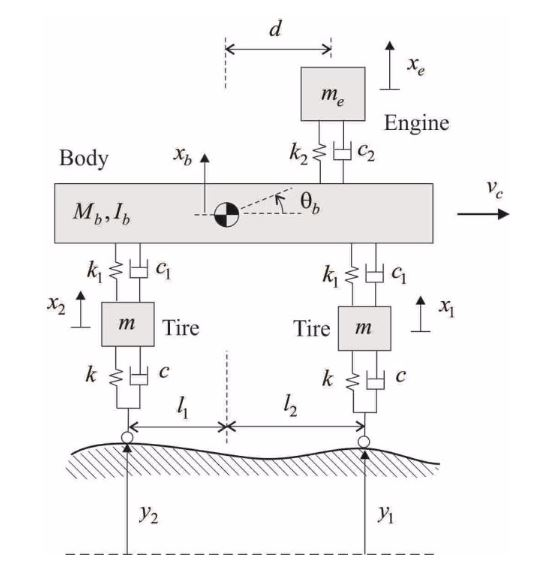
\includegraphics[scale=0.7]{CarModel}
\caption{Five dof model for car}
\end{figure}

\textbf{Note}: The program named \textit{Kanale\_AME521Project\_Task1.m} is written to carry out all the necessary computations for this task. 

\subsection{Solution (1a)- Derive Linear Equations of Motion}
Lagrangian Equations of Motion are given by
\begin{equation}
 \frac{d}{dt} \left( \pdv{L}{\dot{q}_i} \right) - \pdv{L}{q_i} + \pdv{R}{\dot{q}_i} = Q_i
\end{equation}
where $q_i$ is the generalized coordinate, $Q_i$ is the total non-conservative generalized force and $L$ is the Lagrangian given by $L=T-V$ with $T$, $V$ being the Kinetic and Potential energies of the system, respectively. In this case, the generalized coordinates are chosen to be $x_1$, $x_2$, $x_b$, $\theta_b$ and $x_e$.

\textbf{\textit{Effect of Rotation}}:
\noindent
As the body rotates, the front tire, rear tire and the engine have different displacements (and hence, velocities). These displacements are defined as $x_f$, $x_r$ and $x_t$ for the front, rear and engine respectively. From geometry, they are expressed as follows:
\begin{align}
x_f &= x_b + l_2 sin(\theta_b) \\
x_r &= x_b - l_1 sin(\theta_b) \\
x_t &= x_b + d sin(\theta_b)
\end{align}
\noindent
and their linearized derivatives are hence obtained as
\begin{align}
\dot{x}_f &= \dot{x}_b + l_2 cos(\theta_b) \dot{\theta_b} \\
&= \dot{x}_b + l_2 \dot{\theta_b}\\
\dot{x}_r &= \dot{x}_b - l_1 cos(\theta_b) \dot{\theta_b} \\
&= \dot{x}_b - l_1 \dot{\theta_b}\\
\dot{x}_t &= \dot{x}_b + d cos(\theta_b) \dot{\theta_b}\\
&= \dot{x}_b + d  \dot{\theta_b}
\end{align}

\textbf{\textit{Calculate $T$, $V$ and $Q_i$}}: Now, the total Kinetic and Potential Energies, and the Rayleigh's dissipation function of the system are expressed as:
\begin{align}
 T &= \frac{1}{2} \left[ m (\dot{x}_1^2 + \dot{x}_2^2) + M_b \dot{x}_b^2 + \nu_c^2 + I_b \dot{\theta}_b^2 + m_e^2 \dot{x}_e^2 \right] \\[1pt]
 V &= \frac{1}{2} \left[ k(x_1-y_1)^2 + k(x_2-y_2)^2 + k_1(x_r - x_2)^2 + k_1(x_f - x_1)^2 + k_2(x_e - x_t)^2 \right] \\[1pt]
 R &= \frac{1}{2} \left[ c(\dot{x}_1-\dot{y_1})^2 + c(\dot{x}_2-\dot{y}_2)^2 + c_1(\dot{x}_r - \dot{x}_2)^2 + c_1(\dot{x}_f - \dot{x}_1)^2 + c_2(\dot{x}_e - \dot{x}_t)^2 \right]
\end{align} \\

\textbf{\textit{Derive Linearized Equations of Motion}}:
Since $T$ depends only on velocity and $V$ depends only on position, the Equations of motion can be simplified to
\begin{equation}
 \frac{d}{dt} \left( \pdv{T}{\dot{q}_i} \right) + \pdv{V}{q_i} + \pdv{R}{\dot{q}_i} = Q_i
\end{equation}
\noindent
To calculate the first term in the equations:
\begin{align}
\frac{d}{dt}\pdv{T}{\dot{x}_1} &= m \ddot{x}_1\\
\frac{d}{dt}\pdv{T}{\dot{x}_2} &= m \ddot{x}_2\\
\frac{d}{dt}\pdv{T}{\dot{x}_b} &= m_b \ddot{x}_b\\
\frac{d}{dt}\pdv{T}{\dot{\theta}_b} &= I_b \ddot{\theta}_b\\
\frac{d}{dt}\pdv{T}{\dot{x}_e} &= m_e \ddot{x}_1
\end{align}
\noindent To calculate the second term in the equations:
\begin{align}
\pdv{V}{x_1} &= k(x_1 - y_1) - k_1(x_b + l_2 \theta_b - x_1) \\
\pdv{V}{x_2} &= k(x_2 - y_2) - k_1(x_b - l_1 \theta_b - x_2) \\
\pdv{V}{x_b} &= k_1 (x_b - l_1 \theta_b - x_2) + k_1(x_b + l_2 \theta_b-x_1) - k_2(x_e - x_b - d \theta_b)\\
\pdv{V}{\theta_b} &= -k_1 l_1 (x_b - l_1 \theta_b - x_2) + k_1 l_2 (x_b + l_2 \theta_b - x_1) - k_2d(x_e-x_b-d \theta_b) \\
\pdv{V}{x_e} &= k_2 (x_e - x_b - d \theta_b)
\end{align}
\noindent To calculate the third term in the equations:
\begin{align}
\pdv{R}{\dot{x}_1} &= c(\dot{x}_1 - \dot{y}_1) - c_1(\dot{x}_b + l_2 \dot{\theta}_b - \dot{x}_1) \\
\pdv{R}{\dot{x}_2} &= c(\dot{x}_2 - \dot{y}_2) - c_1(\dot{x}_b - l_1 \dot{\theta}_b - \dot{x}_2) \\
\pdv{R}{\dot{x}_b} &= c_1 (\dot{x}_b - l_1 \dot{\theta}_b - \dot{x}_2) + c_1(\dot{x}_b + l_2 \dot{\theta}_b-\dot{x}_1) - c_2(\dot{x}_e - \dot{x}_b - d \dot{\theta}_b)\\
\pdv{R}{\dot{\theta}_b} &= -c_1 l_1 (\dot{x}_b - l_1 \dot{\theta}_b - \dot{x}_2) + c_1 l_2 (\dot{x}_b + l_2 \dot{\theta}_b - \dot{x}_1) - c_2d(\dot{x}_e-\dot{x}_b-d \dot{\theta_b}) \\
\pdv{R}{\dot{x}_e} &= c_2 (\dot{x}_e - \dot{x}_b - d \dot{\theta}_b)
\end{align}

There are no non-conservative forces acting on the system, except for damping which is accounted for by $R$, therefore, $Q_i = 0$. Substituting and simplifying, we obtain the equations of motion in the matrix form as:
\begin{equation}
\boldsymbol{M}\ddot{x} + \boldsymbol{C} \dot{x} + \boldsymbol{K} x = \boldsymbol{f}
\end{equation}
where
\[ \textbf{M} = \begin{bmatrix}
m & 0 & 0 & 0 & 0 \\
0 & m & 0 & 0 & 0 \\
0 & 0 & M_b & 0 & 0 \\
0 & 0 & 0 & I_b & 0 \\
0 & 0 & 0 & 0 & m_e
\end{bmatrix} \]
\[ \textbf{C} =  \begin{bmatrix}
k+k_1 & 0 & -k_1 & -k_1 l_2 & 0 \\
0 & k+k_1 & -k_1 & k_1 l_1 & 0 \\
-k_1 & -k_1 & 2k_1+k_2 & k_2d+k_1 l_2 - k_1 l_1 & -k_2 \\
-k_1l_2 & k_1l_1 & k_2d+k_1l_2-k_1l_1 & k_1l_1^2 + k_1l_2^2 + k_2d^2  & -k_2d \\
0 & 0 & -k_2 & -k_2d & k_2
\end{bmatrix} \]
\[ \textbf{K} =  \begin{bmatrix}
c+c_1 & 0 & -c_1 & -c_1 l_2 & 0 \\
0 & c+c_1 & -c_1 & c_1 l_1 & 0 \\
-c_1 & -c_1 & 2c_1+c_2 & c_2d+c_1 l_2 - c_1 l_1 & -c_2 \\
-c_1l_2 & c_1l_1 & -c_1l_1+c_1l_2+c_2d & c_1l_1^2 + c_1l_2^2 + c_2d^2  & -c_2d \\
0 & 0 & -c_2 & -c_2d & c_2
\end{bmatrix} \]
\[ \textbf{f} = \begin{bmatrix}
c \dot{y}_1 + k y_1 \\
c \dot{y}_2 + k y_2\\
0\\
0\\
0
\end{bmatrix} \]
\textit{Check}: It is seen that \textbf{K} and \textbf{C} are symmetric and \textbf{M} is diagonal, as expected.

\subsection{Solution (1b)- Determine Eigenvalues and Eigenvectors}
Engine assembly: $$m_e=200 kg, k_2=1.3 \times 10^5 Nm{-1}, c_2=1.02 \times 10^3 kgs^{-1}, d=1.65m$$
Car Body: $$M_b = 1650kg, I_b=2330kgm^2, k_1=2.5 \times 10^5Nm^{-1}, c_1=2.73 \times 10^3 kgs^{-1}$$
Tire-Rim Assembly: $$m=75kg, k=2.5 \times 10^5Nm^{-1}, c=1.48 \times 10^3 kgs^{-1}, l_1=1.4m, l_2=1.3m$$
Substituting these values, we get
\[ \textbf{M} = \begin{bmatrix}
75 & 0 & 0 & 0 & 0 \\
0 & 75 & 0 & 0 & 0 \\
0 & 0 & 1650 & 0 & 0 \\
0 & 0 & 0 & 2330 & 0 \\
0 & 0 & 0 & 0 & 200
\end{bmatrix} \]
\[ \textbf{C} =  \begin{bmatrix}
4210 & 0 & -2730 & -3549 & 0 \\
0 & 4210 & -2730 & 3822 & 0 \\
-2730 & -2730 & 6480 & 1410 & -1020 \\
-3549 & 3822 & 1410 & 12741  & -1683 \\
0 & 0 & -1020 & -1683 & 1020
\end{bmatrix} \]
\[ \textbf{K} =  1000 \begin{bmatrix}
500 & 0 & -250 & -325 & 0 \\
0 & 500 & -250 & 350 & 0 \\
-250 & -250 & 630 & 189.5 & -130 \\
-325 & 350 & 189.5 & 1266.4  & -214.5 \\
0 & 0 & -130 & -214.5 & 130
\end{bmatrix} \]

\noindent
Using matlab, it was verified that $$ \boldsymbol{C} \boldsymbol{M}^{-1} \boldsymbol{K} \neq \boldsymbol{K} \boldsymbol{M}^{-1} \boldsymbol{C} $$
which indicates that the system is not proportionally damped.

Therefore, state-space formulation will be used to calculate the eigenvalues and eigenvectors of this ssytem. Which is as follows:
\begin{align}
\boldsymbol{M}\ddot{x} + \boldsymbol{C} &\dot{x} + \boldsymbol{K} x = \boldsymbol{f} \\
\ddot{x} = &\boldsymbol{M}^{1} (\boldsymbol{f}- \boldsymbol{C} \dot{x} - \boldsymbol{K} x)
\end{align}
State vector is defined as:
\[ \textbf{z} = \begin{bmatrix}
x \\
\dot{x}
\end{bmatrix} \implies \boldsymbol{\dot{z}} = \begin{bmatrix}
\dot{x} \\
\ddot{x}
\end{bmatrix} = \begin{bmatrix}
\textbf{O} & \textbf{I} \\
-\textbf{M}^{-1} \textbf{K} & -\textbf{M}^{-1} \textbf{C}
\end{bmatrix} \begin{bmatrix}
x \\
\dot{x}
\end{bmatrix} + \begin{bmatrix}
\textbf{O} \\
-\textbf{M}^{-1} \textbf{f}
\end{bmatrix}
\]
This can be written as: 
\begin{align}
\boldsymbol{\dot{z}} &= \boldsymbol{A} \boldsymbol{z} + \boldsymbol{q} \\
EVP: \quad \boldsymbol{\dot{z}} &= \boldsymbol{A} \boldsymbol{z}
\end{align}
\noindent
\textbf{Note}: Please check the variables \textit{eVecDamp} and \textit{eValDamp} after running the matlab program. The matrices were too big to fit into this sheet

As expected, this system has $2n$ eigen values and $2n$ eigenvectors. 

\subsection{Solution (1c)- Ignore damping and show Eigenvectors are orthogonal}

The equation of motion is then $$\boldsymbol{M}\ddot{x}+\boldsymbol{K}x = \boldsymbol{f}$$
The eigen vectors were determined to be:
\[ \textbf{v}_1 = \begin{bmatrix}
 0.777 \\
0.640 \\
-0.033 \\
-0.002 \\
0.004
\end{bmatrix}, \textbf{v}_2 = \begin{bmatrix}
-0.640 \\
0.766 \\
-0.002 \\
0.032 \\
-0.005
\end{bmatrix}, \textbf{v}_3 = \begin{bmatrix}
-0.201 \\
0.056 \\
-0.133 \\
-0.164 \\
0.956 \\
\end{bmatrix}, \textbf{v}_4 = \begin{bmatrix}
-0.320 \\
-0.049 \\
-0.372 \\
-0.198 \\
-0.847
\end{bmatrix}, \textbf{v}_5 = \begin{bmatrix}
-0.075 \\
0.591 \\
0.479 \\
-0.481 \\
-0.430
\end{bmatrix}
\]
It was verified using matlab that, for $i \neq j$,
\begin{align}
 \boldsymbol{v}_i^T \boldsymbol{M} \boldsymbol{v}_j &= 0 \\ \boldsymbol{v}_i^T \boldsymbol{K} \boldsymbol{v}_j &= 0
\end{align}
\textbf{Note}: \textit{In the code, check the matrix prodMat, where each element (i,j) corresponds to the product of eigen vectors i and j.}

Hence, the eigencvectors of the undamped system are orthogonal.

\subsection{Solution (1d)- Frequency response of Engine assembly($x_e$)}

Given that
$$ y_1(t) = y_0 \sin(\omega t), \quad y_2(t) = y_0 \sin(\omega (t-t_0))$$
$$where \quad \quad \quad \quad \omega=\frac{v_c}{L_r} \quad t_0=\frac{l_1+l_2}{v_c} \quad y_0 = 0.08m \quad L_r=10m$$

Now,
\begin{align}
 y_1 &= y_0 \sin{\omega t} \\
 \dot{y}_1 &= y_0 \omega \cos{\omega t} \\
 y_2 &= y_0 \sin{\omega(t-t_0)} \\
 &= y_0 [\sin{\omega t}\cos{\omega t_0} - \cos{\omega t} \sin{\omega t_0}] \\
 \dot{y}_2 &= y_0 \omega \cos{\omega(t-t_0)} \\
 &= y_0 \omega [\cos{\omega t}\cos{\omega t_0} + \sin{\omega t} \sin{\omega t_0}]
\end{align}
Therefore, \[\textbf{f} = \begin{bmatrix}
c \dot{y}_1 + k y_1 \\
c \dot{y}_2 + k y_2\\
0\\
0\\
0
\end{bmatrix} = \underbrace{\begin{bmatrix}
k y_0 \\
cy_0\omega\sin{\omega t_0} + k y_0\cos{\omega t_0}\\
0\\
0\\
0
\end{bmatrix}}_{\text q_s(\omega)} \sin{\omega t} + \underbrace{\begin{bmatrix}
c y_0 \omega \\
cy_0\omega\cos{\omega t_0} - k y_0\sin{\omega t_0}\\
0\\
0\\
0
\end{bmatrix}}_{\text q_c(\omega)} \cos{\omega t}
\]
Let the steady state solution be of the form
$$ y_{ss} = Y_s \sin{\omega t} + Y_c \cos{\omega t} $$
Using this to rewrite the EoM, and equating coefficients of $\sin$ and $\cos$ terms in LHS and RHS, we get the following martix equation
\[ \begin{bmatrix}
-\omega^2 \textbf{M} + \textbf{K} & -\omega \textbf{C}\\
\omega \textbf{C} & -\omega^2\textbf{M} + \textbf{K}
\end{bmatrix} \begin{pmatrix}
Y_s \\
Y_c
\end{pmatrix} = \begin{pmatrix}
q_s(\omega) \\
q_c(\omega)
\end{pmatrix}
\]
For which the solution can be obtained by
\[ \begin{pmatrix}
Y_s \\
Y_c
\end{pmatrix} = \begin{bmatrix}
-\omega^2 \textbf{M} + \textbf{K} & -\omega \textbf{C}\\
\omega \textbf{C} & -\omega^2\textbf{M} + \textbf{K}
\end{bmatrix}^{-1} \begin{pmatrix}
q_s(\omega) \\
q_c(\omega)
\end{pmatrix}
\]
where $Y_s$ and $Y_c$ are obtained as
\[ Y_s = \begin{pmatrix}
a1 & a2 & a3 .&.&.&.&.&a_n \\
\end{pmatrix}^T, Y_c = \begin{pmatrix}
b1 & b2 & b3 .&.&.&.&.&b_n \\
\end{pmatrix}^T
\]
It follows that
\begin{equation}
y_{ss} = Y_s \sin{\omega t} + Y_c \cos{\omega t} = A_0 \sin{(\omega t + \phi)}
\end{equation}
and $A_0$ and $\phi$ are obtained using the following relations:
\begin{align}
A_0 &= \sqrt{a_k^2 + b_k^2} \\
\phi &= \tan{\frac{b_k}{a_k}}^{-1}
\end{align}
From matlab, the frequency response of Amplitude and Phase angle were obtained for the engine assembly. They are shown in \textit{Figures} \textit{2} and \textit{3}, respectively.

\begin{figure}[!htbp]
\centering
  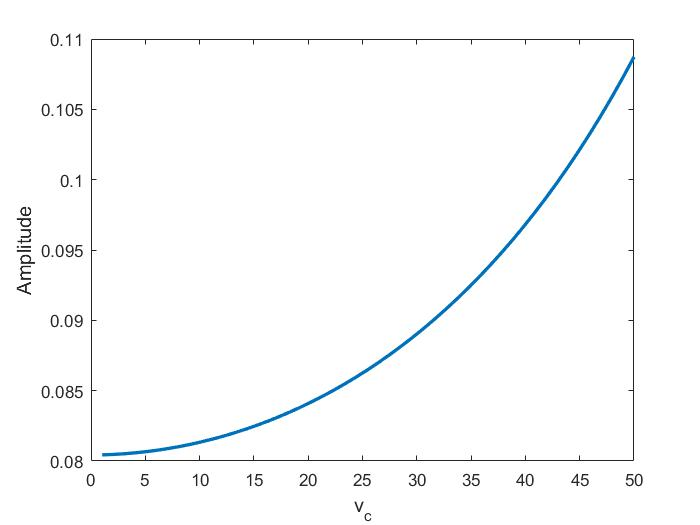
\includegraphics[scale=0.45]{AmplResponse}
  \caption{Amplitude Response}
\end{figure}
\begin{figure}[!htbp]
  \centering
  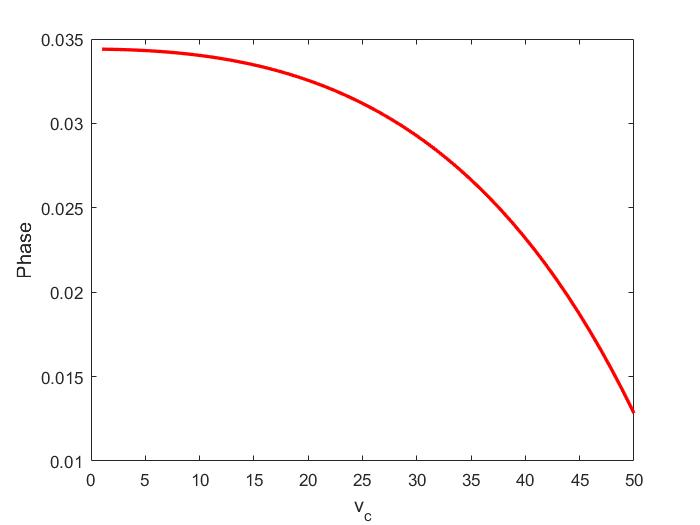
\includegraphics[scale=0.45]{PhResponse}
  \caption{Phase Response}
\end{figure}

\pagebreak
\section{Task 2- A Model of Coupled Vehicle Bridge Systems}
\subsection{Problem Setup}
A car moving on a bridge can be modeled as a moving rigid body coupled to a flexible beam clamped at both ends as show in figures below. The rigid-body and beam are coupled by two pairs of springs and viscous dampers that are a model of the tire-suspension assembly of the car.
\begin{figure}[!htbp]
\centering
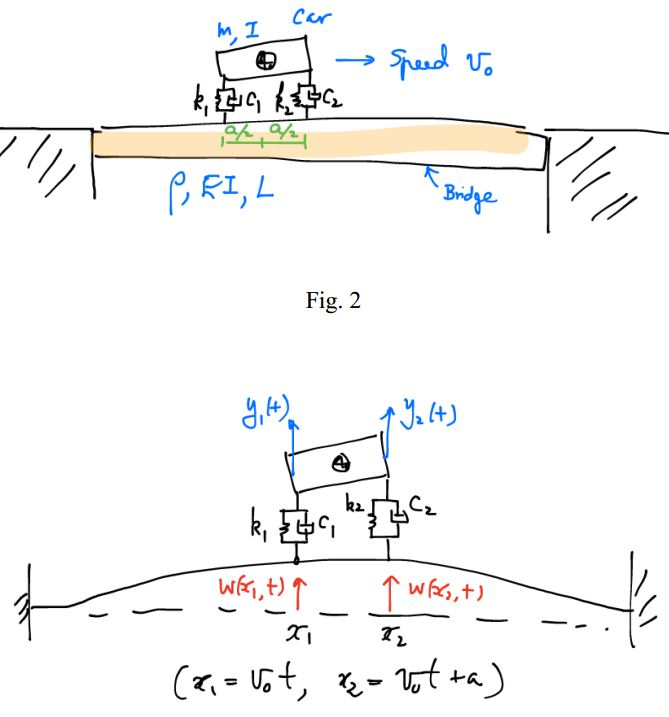
\includegraphics[scale=0.8]{VehicleBridgeModel}
\caption{Vehicle--Bridge coupled system}
\end{figure}

\textbf{Note}: The program named \textit{Kanale\_AME521Project\_Task2.m} is written to carry out all the necessary computations for this task.

 \subsection{Mathematical Model by Assumed Modes method}
The following assumptions are made:
\begin{enumerate}
 \item The effect of gravity on both the beam and rigid body is negligible.
 \item At the initial time $t = 0$, the rear end of the car (the left end of the rigid body) coincides with the left end of the bridge.
 \item The car is moving rightward.
 \item The model is only for the time period $0 \leq t \leq \frac{L-a}{v_0}$. In other words, during this time period, all the tires of the car are within the bridge region ($0 \leq x \leq L$)
\end{enumerate}
The boundary conditions are as follows:
\begin{align*}
w(o,t) &= w(L,t) = 0 \\
w'(0,t) &= w'(L,t) = 0
\end{align*}

Assume $$ w(x,t) \approx \sum_{k=1}^n [\phi_k(x)] \utilde{q}_k(t)$$
where $\phi_k(x) = [\phi_1(x) \quad \phi(v_0t+a)(x) \quad . . . \quad \phi_n(x)]$ is a row vector of the admissible functions of the beam and $\utilde{q}_k(t) = [q_1(x) \quad q_2(x) \quad . . . \quad q_n(x)]^T$ is the column of generalized coordinates.

\begin{enumerate}

\item Kinetic energy can then be expressed as
\begin{align}
 T &= \frac{1}{2} \int_0^L \rho \dot{w}^2 dx + \frac{1}{2}m \left(\frac{\dot{y}_2 + \dot{y}_1}{2}\right)^2 + \frac{1}{2}I\left(\frac{\dot{y}_2 - \dot{y}_1}{a}\right)^2 + \frac{1}{2}mv_0^2 \\
  &= \frac{1}{2}\dot{\utilde{q}}^T [M_b] \dot{\utilde{q}} + \frac{1}{2}m \left(\frac{\dot{y}_2 + \dot{y}_1}{2}\right)^2 + \frac{1}{2}I\left(\frac{\dot{y}_2 - \dot{y}_1}{a}\right)^2 + \frac{1}{2}mv_0^2
\end{align}
where $[M_b] = \int_0^L \rho [\phi(x)]^T [\phi(x)] dx$.

Now write T as,
\begin{align}
  T = \frac{1}{2}\utilde{\dot{q}}_a^T [M_a] \utilde{\dot{q}}_a \\
  \delta T = \utilde{\dot{q}}_a^T [M_a] \delta\utilde{\dot{q}}_a
\end{align}
where 
\begin{equation}
\utilde{q}_a(t) = \begin{pmatrix}
\utilde{q}(t) \\
y(t)
\end{pmatrix}
\end{equation}
\begin{equation}
[M_a] = \begin{bmatrix}
[M_b] & 0 & 0 \\
0 & \frac{m}{4}+\frac{I}{a^2} & \frac{m}{4}-\frac{I}{a^2} \\
0 & \frac{m}{4}-\frac{I}{a^2} & \frac{m}{4}+\frac{I}{a^2}
\end{bmatrix}
\end{equation}

\item Ignoring gravity, Potential energy can be written as
\begin{align}
 V &=  \frac{1}{2} \int_0^L EI (w'')^2dx + \frac{1}{2} k_1 [y_1(t) - w(v_0t,t)]^2 + \frac{1}{2} k_2 [y_2(t) - w(v_0t+a,t)]^2\\
 &=\frac{1}{2} \utilde{q}^T [K_b] \utilde{q} + \frac{1}{2} k_1 \big[y_1^2 + \utilde{q}^T [\phi_1]^T [\phi_1] \utilde{q} - 2y_1[\phi_1]\utilde{q} \big]+ \\ \notag
  &\qquad \qquad \qquad \qquad +\frac{1}{2} k_2 \big[y_2^2 + \utilde{q}^T [\phi(v_0t+a)]^T [\phi(v_0t+a)]\utilde{q} - 2y_2[\phi(v_0t+a)]\utilde{q} \big] \\
  &= \frac{1}{2}\utilde{\dot{q}}_a^T [K_a] \utilde{\dot{q}}_a 
\end{align}
Therefore,
\begin{equation}
\delta V = \utilde{\dot{q}}_a^T [K_a] \delta \utilde{\dot{q}}_a 
\end{equation}

where 
\begin{equation}
[K_a] = \begin{bmatrix}
[K_b]+k_1\phi_1^T\phi_1+k_2\phi(v_0t+a)^T\phi(v_0t+a) & -k_1\phi_1^T & -k_2\phi(v_0t+a)^T \\
-k_1\phi_1 & k_1 & 0 \\
-k_2\phi(v_0t+a) & 0 & k_2
\end{bmatrix}
\end{equation}

where $[K_b] = \int_0^L EI [\phi(x)'']^T [\phi(x)''] dx $

\item Non-conservative work done
\begin{align}
 \delta W_{nc} &= -c_1(\dot{y}_1 - \dot{w}(v_0t,t))\delta y_1 - c_2(\dot{y}_2 - \dot{w}(v_0t+a,t))\delta y_2 + \\ \notag
  & \qquad \qquad \qquad +c_1(\dot{y}_1 - \dot{w}(v_0t,t))\delta w(v_0t,t)+\\ \notag
  & \qquad \qquad \qquad+c_2(\dot{y}_2 - \dot{w}(v_0t+a,t))\delta w(v_0t+a,t) \\ 
  &= -c_1(\dot{y}_1 - [\phi_1] \dot{\utilde{q}})(\delta y_1-[\phi_1]\delta \utilde{q}(t)) + \\ \notag
  & \qquad \qquad \qquad+ -c_2(\dot{y}_2 - [\phi(v_0t+a)] \dot{\utilde{q}})(\delta y_2-[\phi(v_0t+a)]\delta \utilde{q}(t))
\end{align}
As with Mass and Stiffness terms, this can be written as
\begin{align}  
\delta W_{nc} &= -\utilde{\dot{q}}_a^T [C_a] \delta \utilde{q}_a
\end{align}

where 
\begin{equation}
[C_a] = \begin{bmatrix}
c_1\phi_1^T\phi_1+c_2\phi(v_0t+a)^T\phi(v_0t+a) & -c_1\phi_1^T & -c_2\phi(v_0t+a)^T \\
-c_1\phi_1 & c_1 & 0 \\
-c_2\phi(v_0t+a) & 0 & c_2
\end{bmatrix}
\end{equation}
\end{enumerate}

Using the extended Hamilton's Principle and equations (49), (54) and (59)
\begin{align}
 \int_{t_1}^{t_2} (\delta T -\delta V + \delta W_{nc}	)dt &= 0 \\
 [M_a] \ddot{\utilde{q}_a} + [C_a] \dot{\utilde{q}_a} + [K_a]{\utilde{q}_a} &= 0
\end{align}
are the \textbf{Equations of Motion} of the given system. $[M_a], [C_a]$ and $[K_a]$ are given by eqns (51), (56) and (60).

As in \textit{HW 11 Prob 2}, let us choose an admissible function $\phi_k(x) = 1-\cos{\frac{2k \pi x}{L}}$ since it satisfies all the Boundary Conditions and also gives many zeros in the matrices.

\subsection{Simulation using 3 modes}
Car:
\begin{align}
a = 4.5m, M &= 2.5\times 10^3kg, I = 3.2 \times 10^2kg-m^2 \\
k_1 = k_2 = 5\times 10^5&Nm^{-1}, c_1=c_2 = 3.6 \times 10^3kgs^{-1}, v_0 = 18ms^{-1};
\end{align}

\noindent Bridge:
\begin{align}
\rho = 800kgm^{-1}, EI = 7 \times 10^8 Nm^2, L=400m
\end{align}

\noindent Initial conditions:
\begin{align}
y_1(0) = 0.02 m,\quad & \dot{y}_1(0)=0.6ms^{-1} \\
y_2(0) = 0.05 m,\quad & \dot{y}_2(0)=-0.3ms^{-1}
\end{align}

\noindent Using a 3 term approximation,
\begin{align}
\phi_1(x) &= 1-\cos{\frac{2 \pi x}{L}} \\
\phi_2(x) &= 1-\cos{\frac{4 \pi x}{L}} \\
\phi_3(x) &= 1-\cos{\frac{6 \pi x}{L}}
\end{align}

\noindent Using State space formulation, 
\begin{align}
 z &= \begin{bmatrix}
q_a(t) \\
\dot{q}_a(t)
\end{bmatrix} \\
\implies \dot{z} &= [A(t)] z(t)
\end{align}
where 
\begin{align}
[A(t)] = \begin{bmatrix}
O & I \\
-M_a^{-1} K_a & -M_a^{-1} C_a
\end{bmatrix}
\end{align}
The beam displacements at discrete time intervals, given by $t=k \cdot \Delta t, k=0,1,...6$, are plotted in the figure below.
\begin{figure}[!htbp]
	\centering
	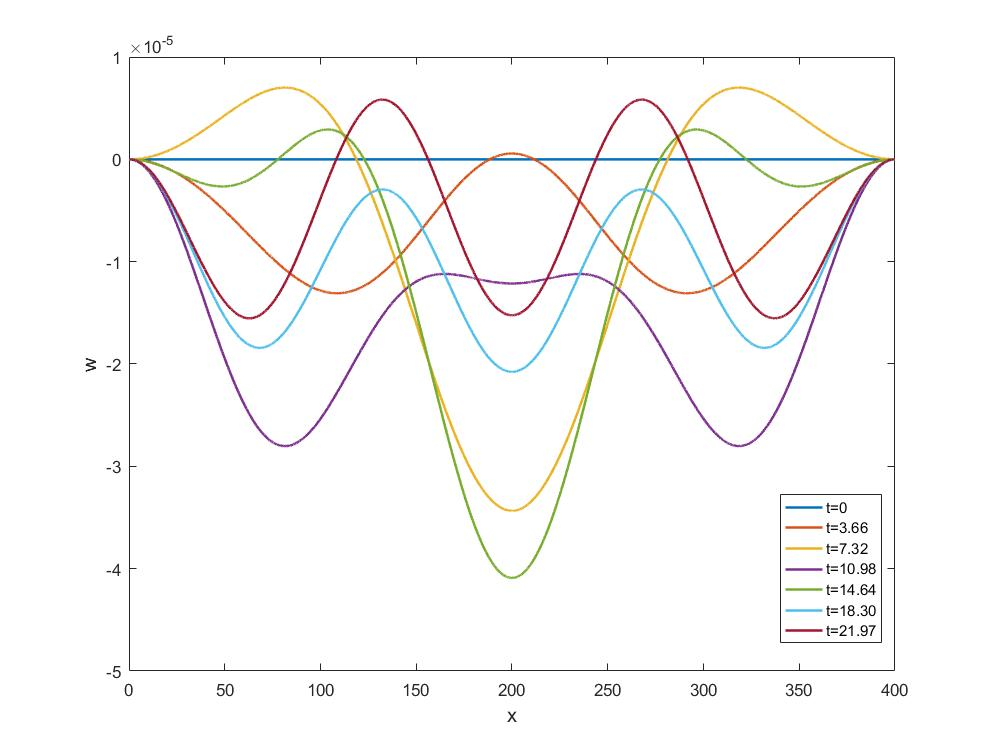
\includegraphics[scale=0.3]{BeamDisp}
	\caption{Beam displacement plot}
\end{figure}

The Vibrational response of the car is shown in figures below. It was intuitively expected that the amplitude gets lower until the vibrations get damped out eventually. This is exactly the behavior seen in the plots.
\begin{figure}[!htbp]
	\centering
	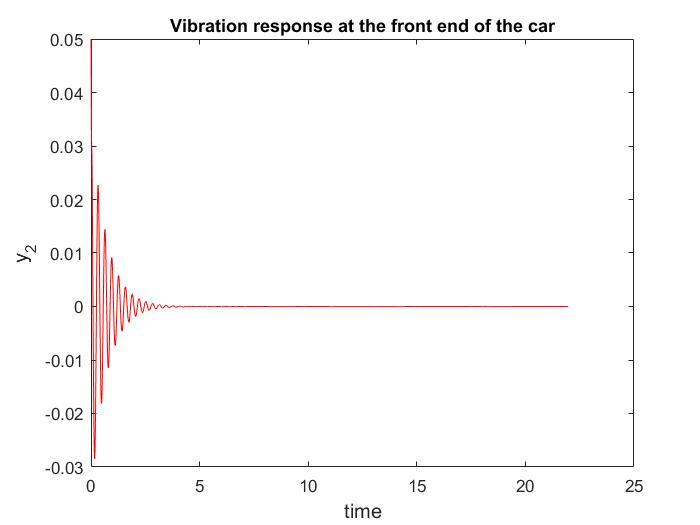
\includegraphics[scale=0.3]{CarVibFront}
	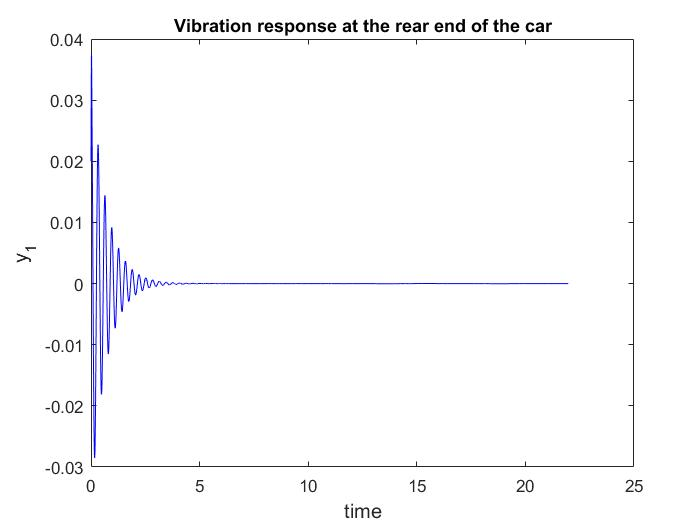
\includegraphics[scale=0.3]{CarVibRear}
	\caption{Vibration Response of the front and rear of the Car moving on a bridge}
\end{figure}

\clearpage
\subsection{Simulation with Impulse Load}
Front tire hits a rock at the middle of the bridge($x=L/2$)
\begin{equation}
 f(t) = I_0 \delta(t-t_{imp})
\end{equation}
with $ I_o=1.2 \times 10^3 kgms^{-1}$ and $t_{imp} = \frac{L-a}{2v_0}$ is applied to the rigid body at the front.

This case is similar to the last case, except for the fact that at the time of impact, i.e., at $t=t_{imp} = \frac{L-a}{2v_0}$ there is an impulse force. Mathematically, 
\begin{align}
\dot{z} &= [A(t)] z(t) + d
\end{align}
where
\begin{align}
d = \begin{pmatrix}
\utilde{O}\\
M_a^{-1} I_0 \delta(t-t_{imp})
\end{pmatrix}
\end{align}
The program can be modified fairly easily in this case. At $t=t_{imp}$ the matrix d is finite whereas it is zero at all other times. 
\begin{figure}[!htbp]
	\centering
	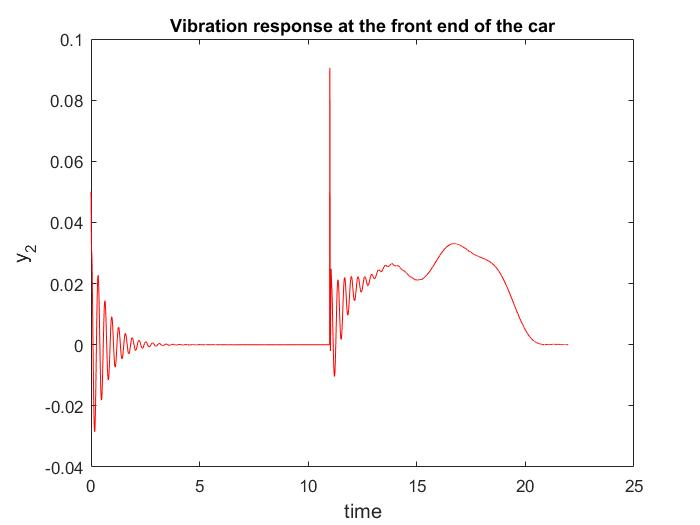
\includegraphics[scale=0.3]{CarVibFront_Impulse}
	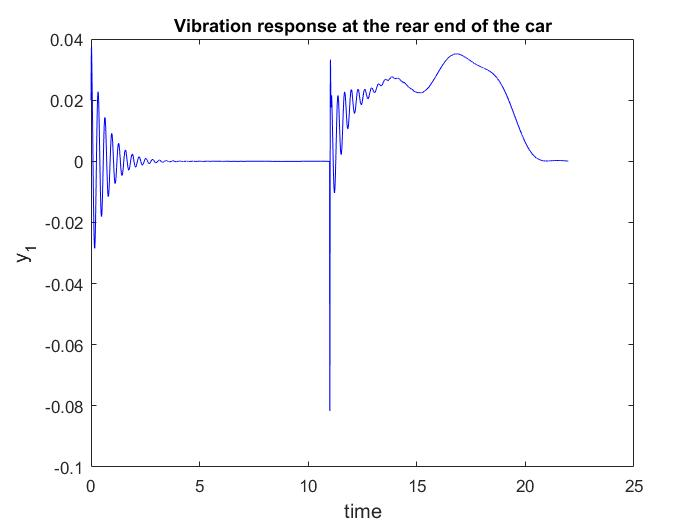
\includegraphics[scale=0.3]{CarVibRear_Impulse}
	\caption{Vibration Response of the front and rear of the Car to an Impulse Load}
\end{figure}

\noindent \textbf{Comparison with No Impulse case}: It is seen (figure 7) that the impulse introduces a perturbation in the front displacement $y_2$, which in turn induces a negative perturbation on the rear wheel, $y_1$. This makes sense as $y_1$ and $y_2$ are coupled in a rotational sense. The system loses stability for some time, before the vibrations die out due to damping as in the previous case. 

\pagebreak
\noindent \textbf{Note}: The beam displacement diagram in the case with impulse is shown in Figure 8. Notice that the beam is also deflected \textit{upward}, due to the impulse. This might seem counter-intuitive, but the reason behind this is probably that in this model, the road and the tires of the car are assumed to be in contact always, i.e. they move as a rigid body. This means that as the tire moves up, it drags the road up along with it.
\begin{figure}[!htbp]
	\centering
	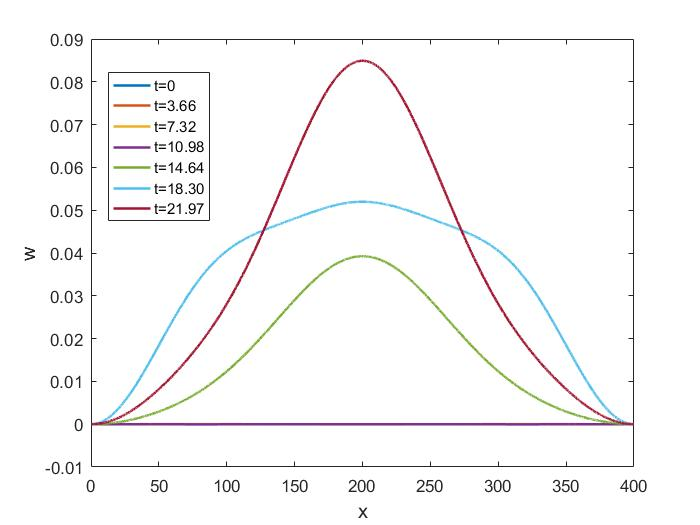
\includegraphics[scale=0.5]{BeamDispImpulse}
	\caption{Beam displacement in the presence of Impulse Load}
\end{figure}
\end{document}